\documentclass[12pt]{article}
\usepackage[english]{babel}
\usepackage[utf8x]{inputenc}
\usepackage{amsmath, subfigure, float}
\usepackage{graphicx}
\usepackage{graphicx, lipsum,caption}
\usepackage[colorinlistoftodos]{todonotes}

\begin{document}
	
	\begin{titlepage}
		
		\newcommand{\HRule}{\rule{\linewidth}{0.5mm}} % Defines a new command for the horizontal lines, change thickness here
		
		\center % Center everything on the page
		
		%----------------------------------------------------------------------------------------
		%	HEADING SECTIONS
		%----------------------------------------------------------------------------------------
		
		\textsc{\LARGE Central Washington University}\\[1.5cm] % Name of your university/college
		\textsc{\Large Circular Coordinate Visualization Software}\\[0.5cm] % Major heading such as course name
		\textsc{\large Winter 2019}\\[0.5cm] % Minor heading such as course title
		
		%----------------------------------------------------------------------------------------
		%	TITLE SECTION
		%----------------------------------------------------------------------------------------
		
		\HRule \\[0.4cm]
		{ \huge \bfseries User Manual}\\[0.4cm] % Title of your document
		\HRule \\[1 cm]
		
		%----------------------------------------------------------------------------------------
		%	AUTHOR SECTION
		%----------------------------------------------------------------------------------------
		
		\begin{minipage}{0.4\textwidth}
			\begin{flushleft} \large
				\emph{Authors:}\\
				Michael \textsc{Brice}\\ % Your name
				Jia \textsc{Song} \\% Your name
				Brian \textsc{Hooper}\\ % Your name
				Hermann \textsc{Yepdjio}\\ % Your name
			\end{flushleft}
		\end{minipage}
		~
		\begin{minipage}{0.4\textwidth}
			\begin{flushright} \large
				\emph{Supervisor:} \\
				Dr. Boris \textsc{Kovalerchuck} % Supervisor's Name
			\end{flushright}
		\end{minipage}\\[1cm]
		
		% If you don't want a supervisor, uncomment the two lines below and remove the section above
		%\Large \emph{Author:}\\
		%John \textsc{Smith}\\[3cm] % Your name
		
		%----------------------------------------------------------------------------------------
		%	DATE SECTION
		%----------------------------------------------------------------------------------------
		
		{\large \today}\\ % Date, change the \today to a set date if you want to be precise
		
		%----------------------------------------------------------------------------------------
		%	LOGO SECTION
		%----------------------------------------------------------------------------------------
		
		
\includegraphics[width=10cm]{CWU-Logo.png}\\[.5cm] % Include a department/university logo - this will require the graphicx package
		
		%----------------------------------------------------------------------------------------
		
		\vfill % Fill the rest of the page with whitespace
		
	\end{titlepage}
	\newpage
	\tableofcontents
	\newpage
	
	
	\section{Format and Type of File Required}
		The Circular-Coordinate supports .csv files only. The .csv file must be formatted as follow
			\begin{itemize}
				\item the first column contains the indexes for all the  entries 
				\item the last column contains the class labels for all the entries
				\item the first row contains the labels for each column
			\end{itemize}
		
		Below is an example of what the .csv file should look like.\\
		
			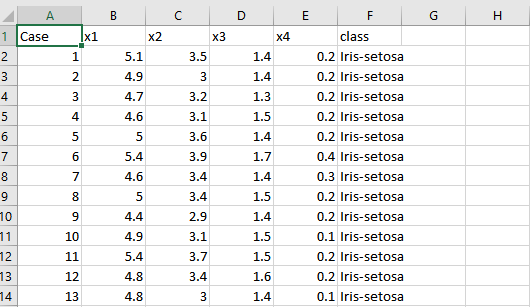
\includegraphics[width=10cm]{csv.png}\\
			Figure 1: An example of what the .csv file should look like
			
	\section{Load a Data Set}
		To load a file
		\begin{itemize}
			\item Select "File" on the upper left corner of the main window and then "Open" or press "Ctrl + O" on the keyboard. 
			\item A window will open. Navigate and select the file containing the data which you want to visualize and press "open".
			
			\begin{figure}[H]
				\hfill
				\subfigure[Open File]{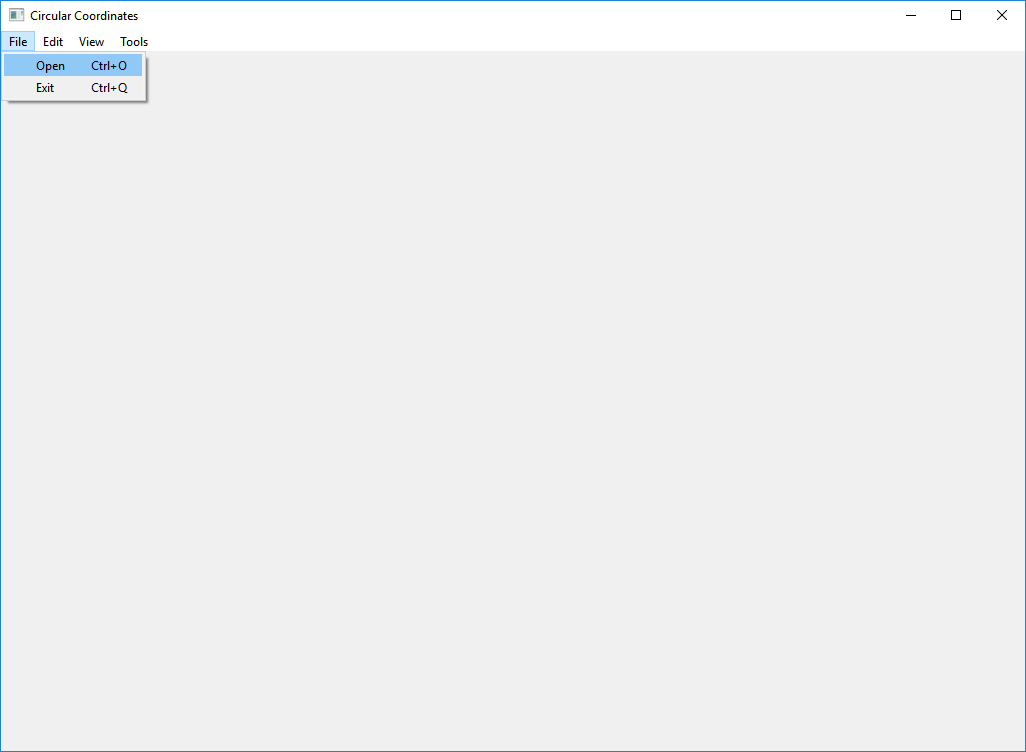
\includegraphics[width=6cm]{open_file.png}}
				\hfill
				\subfigure[Select File]{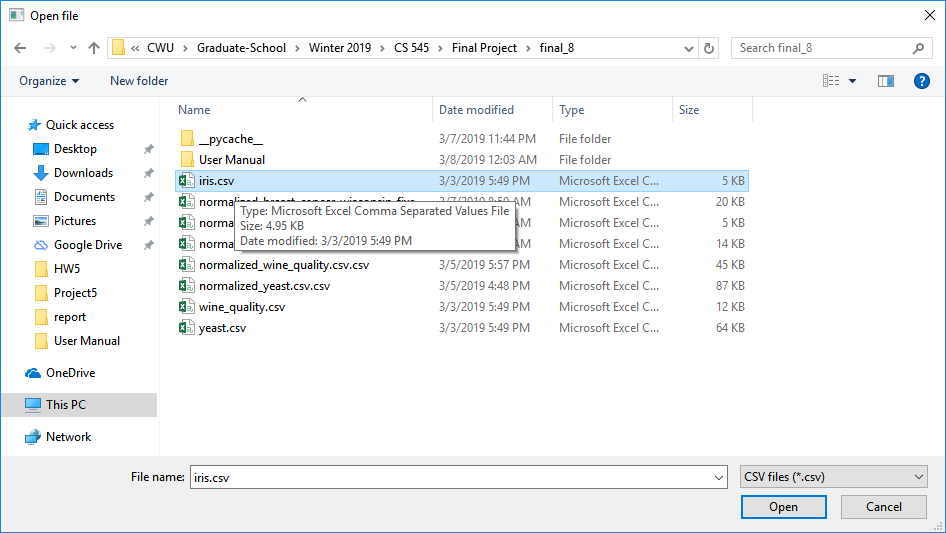
\includegraphics[width=6cm]{select_file.png}}
			\end{figure}
			\centering{Figure 2.}\\
			
			If  the steps above were performed properly, a visualization (in the circular coordinate) of the data that you provided will appear on the main window.\\
			
			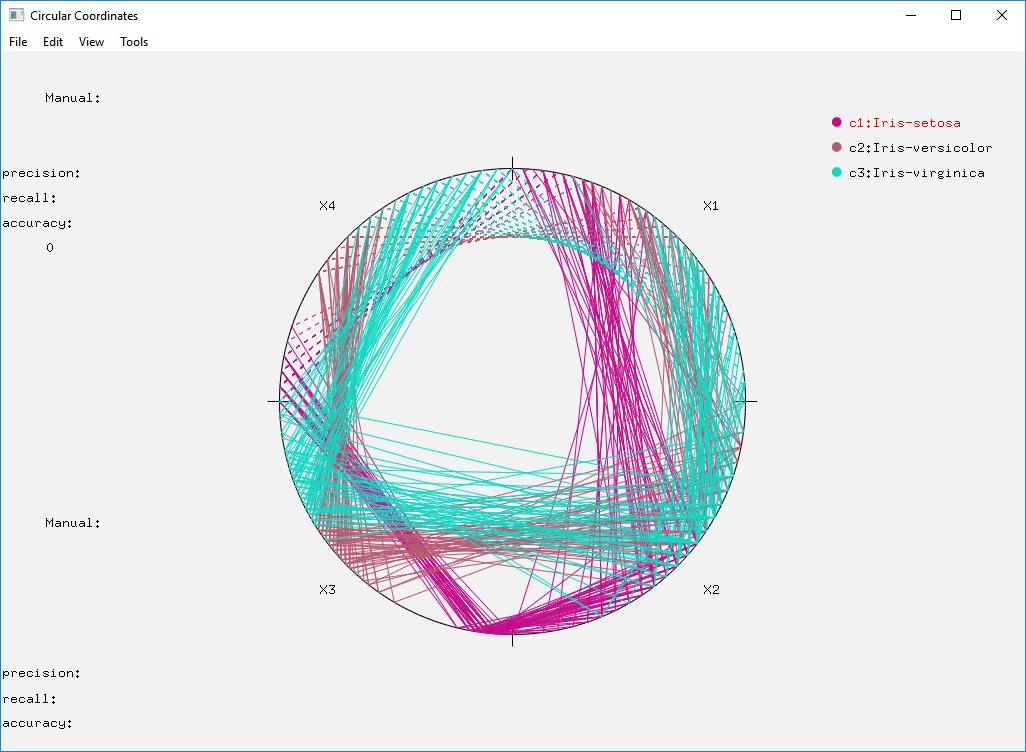
\includegraphics[width=8cm]{main_screen.png}\\
			Figure 3. A visualization of the famous\\
			Iris data set in the circular coordinate
		\end{itemize}
	
	\section{The components of the main window}
		As seen in Figure 3, the main windows contains:
		\begin{itemize}
			\item A confusion matrix along with its corresponding statistics on the upper left corner, for the dominant rectangle that are drawn automatically.
			\item A confusion matrix along with its corresponding statistics on the lower left corner, for the dominant rectangle that are drawn manually.
			\item The list of classes on the right upper corner
		\end{itemize}
		
		
		
	\section {Change the colors of the classes}
		There are 2 ways to change the colors: 
		\begin{itemize}
			\item Randomly by pressing the "r" key on the keyboard.
			\item Manually by selecting "Tools" on the menu bar, then "Set class color" and then select a color. Doing this will change the color of the highlighted class to the color you chose.
		\end{itemize}
	
	\section{The Dominant Rectangles}
		There are two ways to draw the dominant rectangles:
		\begin{itemize}
			\item manually by clicking once with the left button of the mouse to set one point of diagonal of the rectangle. Left-clicking the second time will set the second point of the diagonal and a rectangle will be drawn with the color of the highlighted class. (Right clicking will erase the manually drawn rectangle of the highlighted class) 
			\item automatically by pressing the key "d" on the keyboard.
		\end{itemize}	
		
		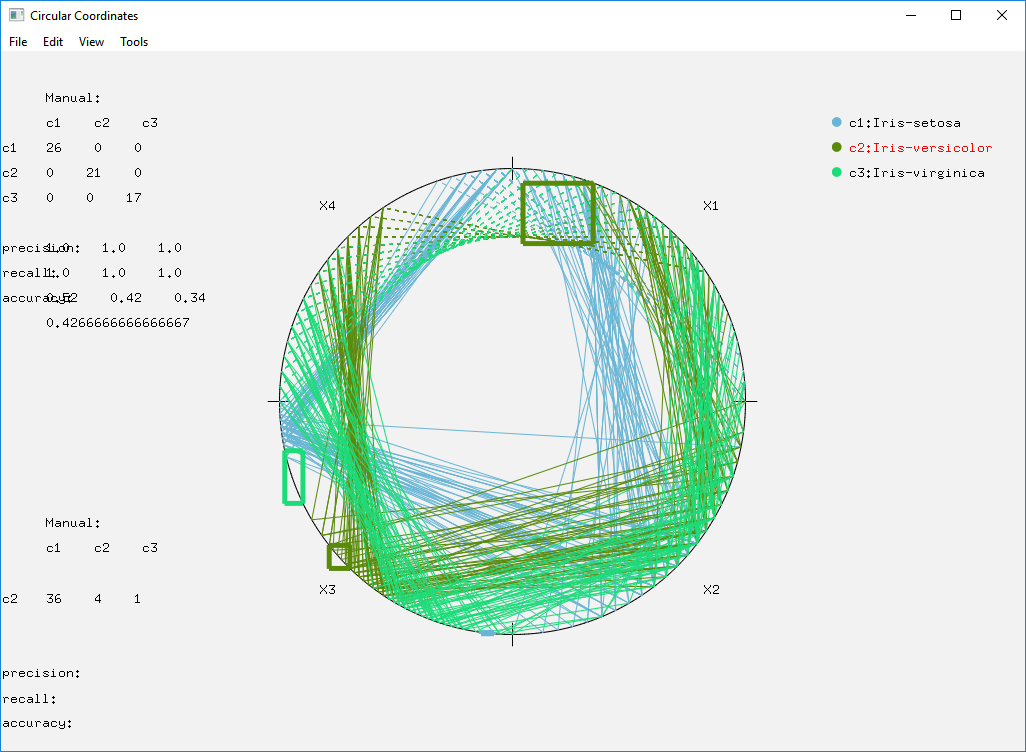
\includegraphics[width=8cm]{dominant_rectangles.png}\\	
	
	\section{Other Options}
		In addition to the functionalities described above, it is also possible to :
		\begin{itemize}
			\item reverse coordinates for better distinction between classes by pressing "X + number" (number being any number from 0 to 9)
			\item navigate through the classes using arrow keys. if "Enter" is pressed, the selected class will be disabled if it was enabled and enabled if it was disabled.
			\item erase all the manually drawn dominant rectangle by selecting "Tools", then "Clear rectangles" or pressing "Ctrl + W" on the keyboard
		\end{itemize}
		
	
\end{document}
